%\documentclass[12pt, letterpaper, twoside]{article}
\documentclass[12pt, letterpaper]{article}
 
\usepackage{amssymb,longtable,dcolumn}
% to use pdflatex
% Standard bbing packages
\usepackage{cite}      % Written by Donald Arseneau
\usepackage{graphicx}  % Written by David Carlisle and Sebastian Rahtz
\usepackage{url}       % Written by Donald Arseneau
\usepackage{amssymb,longtable,dcolumn}
%\usepackage{subfigure}
%\usepackage{stfloats}  % Written by Sigitas Tolusis
\usepackage[caption=false,font=footnotesize]{subfig}
%\usepackage{fixltx2e}
\usepackage{colortbl}
\usepackage{multirow}
\usepackage{amsmath}
\usepackage{units}
\usepackage{color,soul}
\usepackage[margin=1in]{geometry}


\title{Discrete Lowpass Filters}
\author{Brian Bingham}% \thanks{}}
\date{December 2016}
\begin{document}

%\begin{titlepage}
\maketitle
%\end{titlepage}

\section*{Introduction}
Digital (finite-difference) implementation first and second-order lowpass filters for use in control.

\section{First-Order Lowpass}
\subsection{Analog Form}
We can write the transfer function for a first-order lowpwass filter as
\[
H(s) = \frac{Y(s)}{X(s)} = \frac{1}{(\tau)s +1} = \frac{\omega_c}{s+\omega_c}
\]
where $\tau$ is the time constant in seconds and $\omega_c$ is the cut-off freuency in rad/s.
\subsection{Discrete Euler Implementation}
The discrete approximation of this filter is often written as
\[
y[k] = (1-\alpha) y[k-1] + (\alpha) x[k]
\]
where the smoothing factor $0 \leq \alpha \leq 1$ is
\begin{eqnarray*}
\alpha & = & \frac{\Delta t}{\tau + \Delta t} = \frac{1}{1+(\tau / \Delta t)}\\
       & = & \frac{\omega_c (\Delta t)}{(\omega_c (\Delta t)+1)}.
\end{eqnarray*}
This implementation can be derived using the ``backward rectangular rule'' for numerical integration of the original ODE.


Working backwards we can define the discrete-time (z-domain) transfer function for this as
\[
H(z) = \frac{\alpha}{1 + (1-\alpha)z^{-1}}.
\]

\begin{itemize}
\item \url{http://web.cecs.pdx.edu/~tymerski/ece452/6.pdf}
\item \url{https://en.wikipedia.org/wiki/Low-pass_filter#Discrete-time_realization}
\item \url{http://techteach.no/simview/lowpass_filter/doc/filter_algorithm.pdf}
\end{itemize}

\subsection{Bilinear Transform}
An alternate form is derived is we apply the bilinear transform to the original transfer function.  Write the transfer function in normalized form
\[
H(s) = \frac{1}{\left(\frac{s}{\omega_{ac}}\right)+1}
\]
Apply a pre-warping transformation to calculate the equivalent analog cut-off frequency
\[
\omega_{ac} = \tan{\left(\frac{\omega_c (\Delta t)}{2}\right)}
\]
and let
\[
c = \frac{1}{\omega_{ac}}=\cot{\left(\frac{\omega_c (\Delta t)}{2}\right)}
\]
Substitute 
\[
H(s) = \frac{1}{(c)s+1}
\]
Apply bilinear transform using $s=(1-z^{-1})/(1+z^{-1})$
\[
H(z) = \frac{1}{c\left(\frac{1-z^{-1}}{1+z^{-1}}\right)+1}
\]
\[
H(z) = \frac{1 + z^{-1}}{(1+c)+(1-c)z^{-1}}
\]
then covert to a difference equation
\[
y[k] = \frac{1}{c+1} \left[ (1-c) y[k-1] + x[k] + x[k-1] \right]
\]
which agrees wtih the coefficients listed at \url{http://www.apicsllc.com/apics/Sr_3/Sr_3.htm}.

\begin{itemize}
\item \url{https://ocw.mit.edu/courses/mechanical-engineering/2-161-signal-processing-continuous-and-discrete-fall-2008/lecture-notes/lecture_19.pdf}
\end{itemize}


\section{Second-Order Butterworth Filter}
\subsection{Analog Form}
We can write the transfer function for the normalized frequency $a=\frac{s}{\omega_c}$ where $\omega_c$ is the cut-off frequency in rad/s as
\[
H(a) = \frac{1}{a^2 + (\sqrt{2}) a + 1}.
\]
This can then be written in terms of the of $\omega_c$ as
\[
H(s) = \frac{\omega_c^2}{s^2 + (\sqrt{2})\omega_c s + \omega^2}
\]
The frequency response of this analog transfer function is shown in Figure~\ref{f:butter}
\begin{figure}[ht!]
\centering
{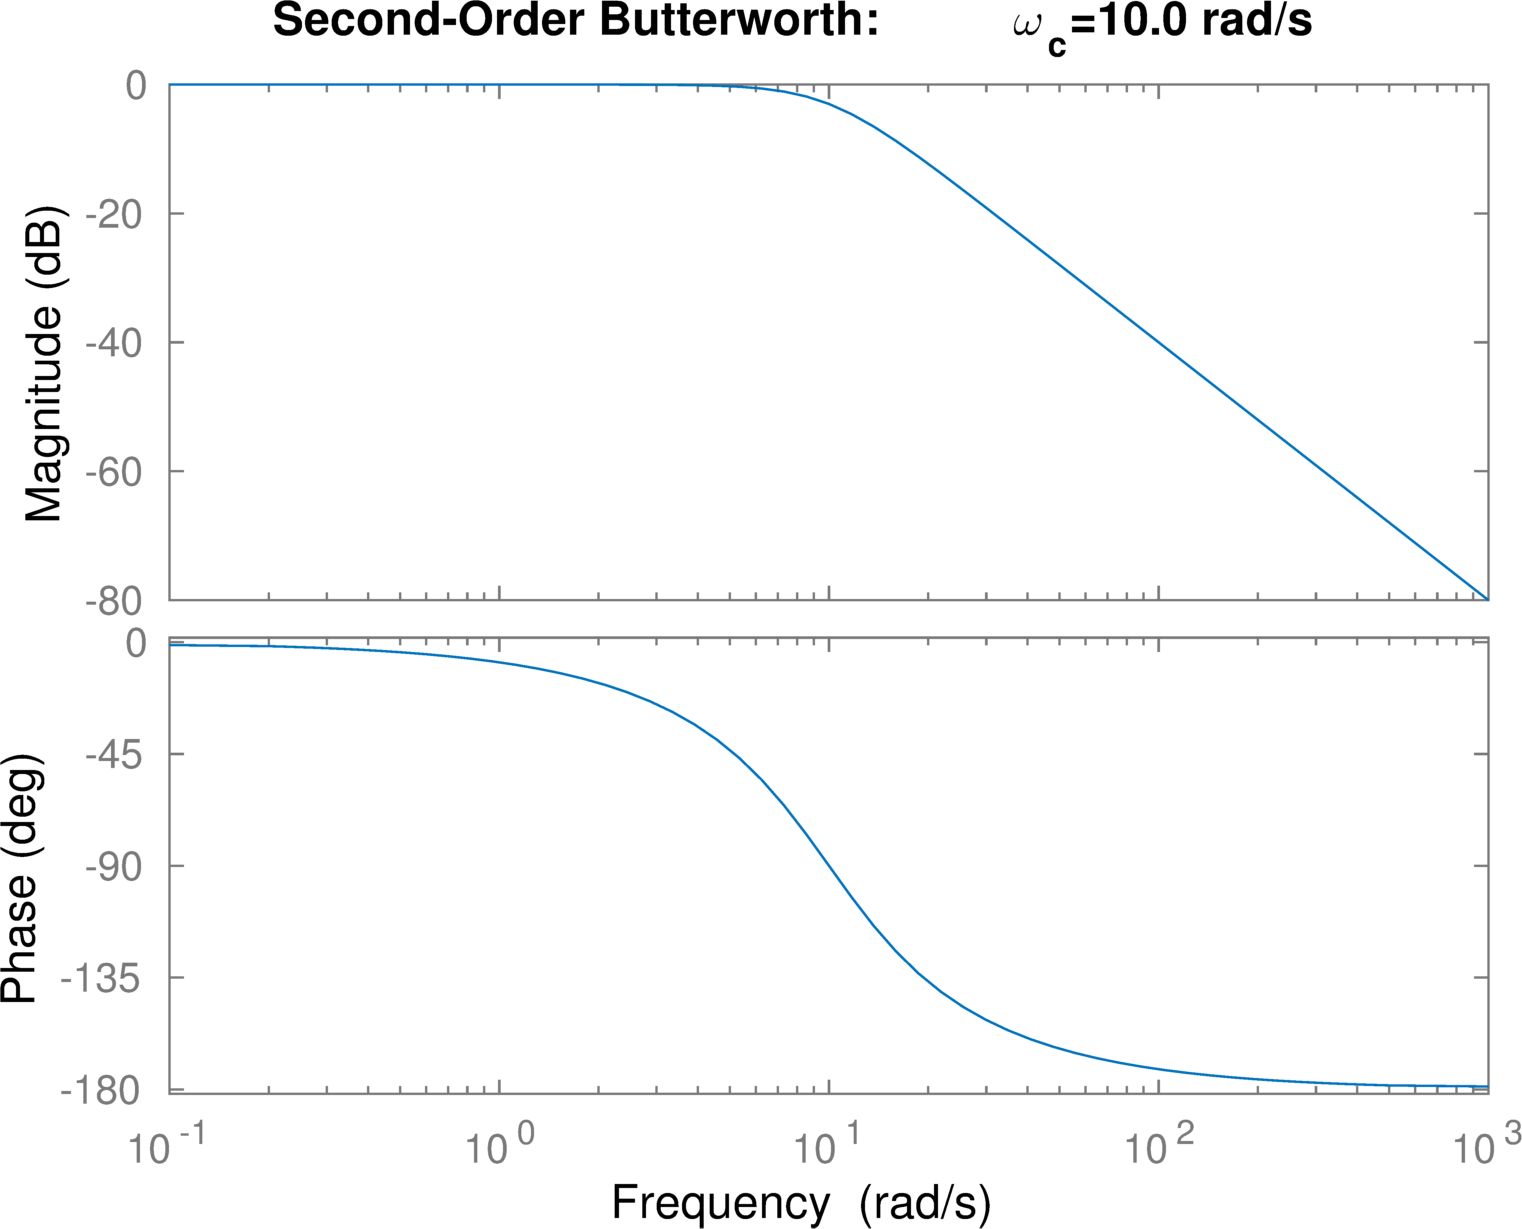
\includegraphics[width=0.75\textwidth]{butter_2.png}}
\caption{Analog frequency response.}
\label{f:butter}
\end{figure}

\section{Digital Form}
The general second-order IIR filter can be expressed as
\[ 
H(z) = \frac{n_0+n_1 z^{-1} + n_2 z^{-2}}{d_0 +d_1 z^{-1}+d_2 z^{-2}}.
\]
The resulting difference equation, assuming $x[k]$ as input and $y[k]$ as output is
\[
y[k] = \frac{1}{d_0}\left[ -d_1 (y[k-1]) -d_2(y[k-2]) + n_0(x[k]) + n_1(x[k-1]) + n_2 (x[k-2])\right]
\]
For the Butterworth low-pass filter the coefficicients are
\begin{eqnarray*}
n_0 & = & 1 \\
n_1 & = & 2 \\
n_2 & = & 1 \\
d_0 & = & c^2+(\sqrt{2})c+1 \\ 
d_1 & = & -2(c^2-1) \\ 
d_2 & = & c^2-(\sqrt{2})c+1 \\ 
\end{eqnarray*}
where
\[
c = \cot{\left(\frac{\omega_c (\Delta t)}{2}\right)}
\]
is the inverse of the pre-warped equivalent cut-off frequency\footnote{\url{https://www.staff.ncl.ac.uk/oliver.hinton/eee305/Chapter5.pdf}}
\[
\omega_{ac} = \tan{\left(\frac{\omega_c (\Delta t)}{2}\right)}
\]
and $\Delta t$ is the sample time in seconds.  See \url{http://www.apicsllc.com/apics/Sr_3/Sr_3.htm}.

Making the substitution we arrive at
%\[
%\begin{split}
\begin{multline*}
y[k] = \frac{1}{(c^2+(\sqrt{2})c+1)} \biggl[ 2(c^2-1)(y[k-1]) -(c^2-(\sqrt{2})c+1)(y[k-2])  \\
+ x[k] + 2(x[k-1]) + x[k-2]\biggr]
%end{split}
%]
\end{multline*}

\subsection{Derivation of General Second Order Butterworth Filter}
Start with the general analog Butterworth transfer function.
\[
H(s) = \frac{\omega_c^2}{s^2 + (\sqrt{2})\omega_c s + \omega_c^2}
\]
Put into normalized from
\[
H(s) = \frac{1}{\left(\frac{s}{\omega_{ac}}\right)^2 + (\sqrt{2})\left(\frac{s}{\omega_{ac}}\right) + 1}
\]
where $\omega_{ac}$ is the equivalent analog cut-off frequency after pre-warping.
Apply the warping function
\[
\omega_{ac} = \tan{\left(\frac{\omega_c (\Delta t)}{2}\right)}
\]
and let
\[
c = \frac{1}{\omega_{ac}}=\cot{\left(\frac{\omega_c (\Delta t)}{2}\right)}
\]
Substitute $c$ into the transfer function
\[
H(s) = \frac{1}{(cs)^2 + (\sqrt{2})(cs) + 1}
\]
Now perform the bilinear transform by substituting
\[
s = \frac{z-1}{z+1}=\frac{1-z^{-1}}{1+z^{-1}}
\]
to get
\[
H(z) = \frac{ (1+z^{-1})^2 }{ c^2 (1-z^{-1})^2 + (\sqrt{2}) c (1-z^{-1})(1+z^{-1})+(1+z^{-1})^2}
\]
\[
H(z) = \frac{ 1 + 2 z^{-1} + z^{-2} }{ (c^2+(\sqrt{2})c+1) - 2(c^2-1)z^{-1} + (c^2 - (\sqrt{2})c +1) z^{-2}}
\]

\section{Verification and Comparison}
Figure~\ref{f:imp} illustrates the frequency reponse of the three digital filters.  The frequency response is determined from the z-domain transfer funtions.  for the two first-order implementations We can see that the simpler alpha-filter implementation has an equivalent frequency response to the bilinear implementation.  

For the second-order Butterworth filter, the frequncy reponse verifies that the bilinear transform, with pre-warping the critical frequency, reproduces the analog frequency response of the design.
\begin{figure}[ht!]
\centering
{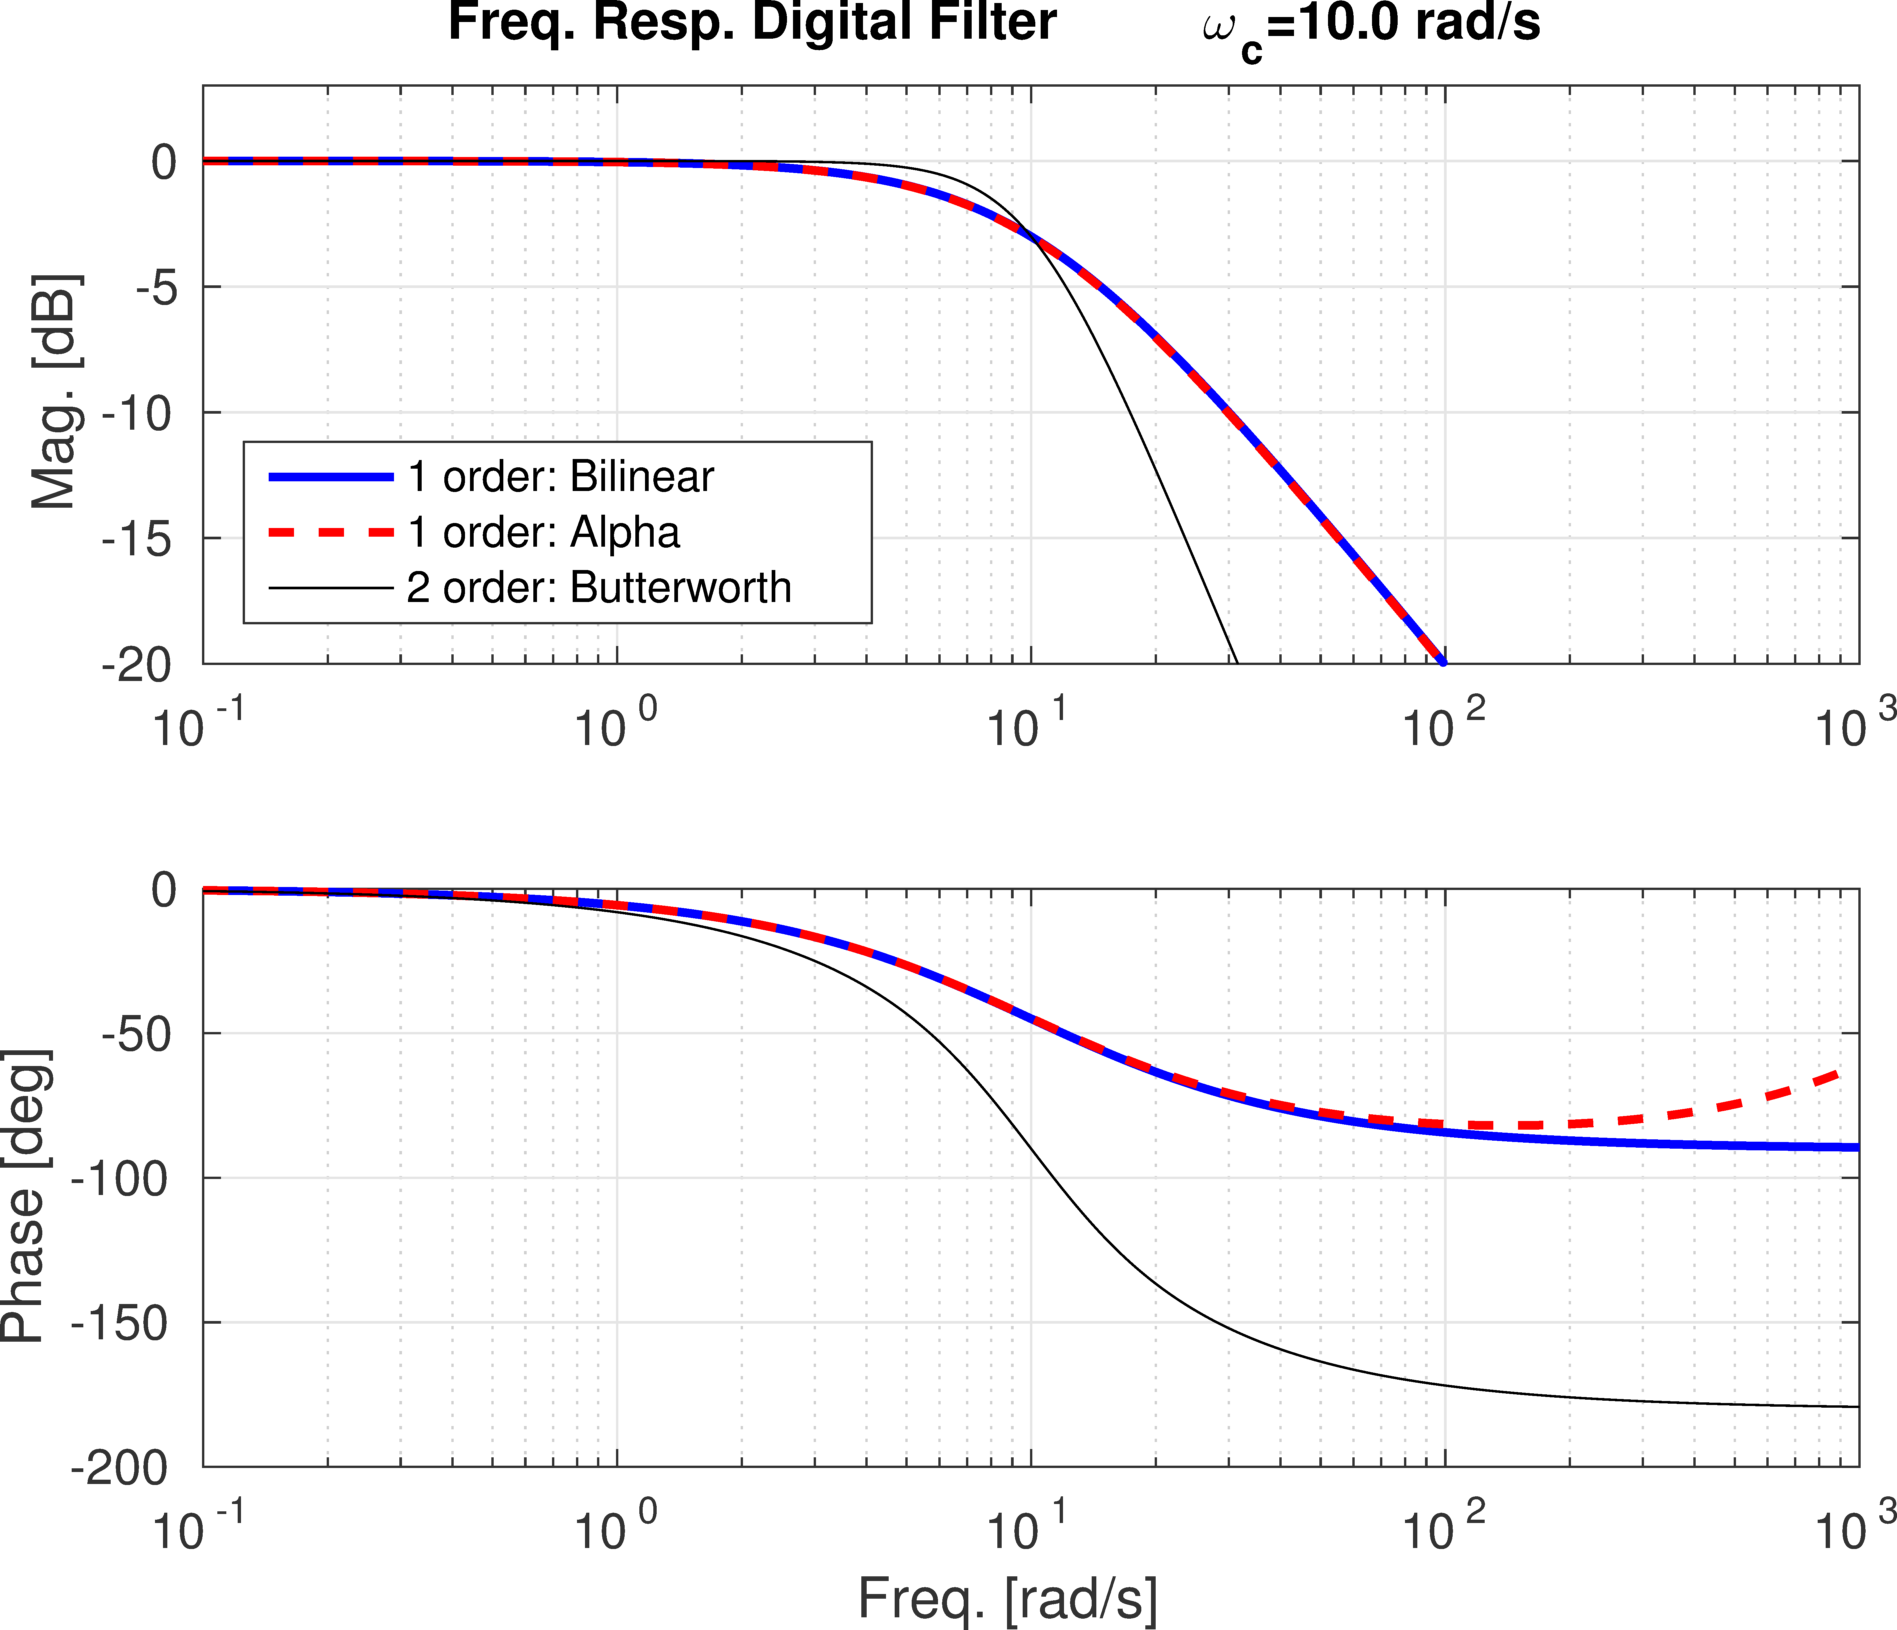
\includegraphics[width=0.75\textwidth]{filter_freqresp.png}}
\caption{Frequency response of digital implementation.}
\label{f:imp}
\end{figure}

\end{document}
